The controller keeps track of all nodes and handles their registration.
It executes the watering policy that the user has selected for each flower.
For this task it wirelessly communicates with the sensor node situated in the flower pot and the pump node situated next to the water tank. The sensor node provides the controller with the most recent measurement values, whereas the pump node executes the pump commands received from the controller.

\subsubsection{State diagram}

\begin{figure}[h!]
	\begin{center}
	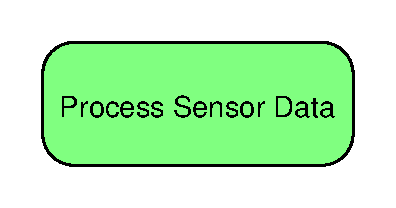
\includegraphics[scale=0.24]{../ControlNode_Diagramm.pdf}
	\caption{Overview of the chosen setup.}
	\label{Setup_overview}
	\end{center}
\end{figure}


States:
\begin{itemize}
	\item Check pending tasks

		This is the begin of the loop() Function. The controller will always come back to this state to check which tasks are pending. The following actions are possible:

		\begin{itemize}
			\item A NRF24 message is arrived, process this message.
			\item Also if an interactive command has arrived via the IOT framework, this command has to be processed. (Typically sending an instruction to a Motor Node)
			\item If, according to the watering schedule, a pump node should take an action now, the controller goes to the ``Send Watering Command to Motor Node'' state
			\item If a Motor Node did not respond as expected, an error handling sequence should be started (writing to log and if needed respond to the IOT framework)
		\end{itemize}

	\item Send Watering Command to Motor Node
		Whenever the controller decides a pump node should start to pump, this function is called. 			It prepares and sends a message to concerned the pump node. It also writes the message content to a log file.
	\item Write Pump Node Timeout to Log
		If a pump node does not reply within the specified timeout duration, an entry into the log file has to be written. In case the command of the concerned message has been triggered by the IOT framework, the controller will move to the ``Send Error Notification to App'' state. Otherwise it enters the ``Reschedule Watering'' state.
	\item Send Error Notification to App
			If a IOT command could not be successfully executed, the IOT framework has to be notified about the problem. Afterwards the controller goes back to checking for pending tasks.
	\item Reschedule Watering
		If a scheduled watering task failed, the controller needs to reschedule this watering task.
		There are many possible algorithms for this such as:
		\begin{itemize}
			\item Skip this watering task and proceed as usual
			\item Retry the watering task a certain number of times. If it fails, proceed as usual
			\item Reschedule the watering of this pump node in a given fashion.
		\end{itemize}
		For a first version it is sufficient to skip the watering, if it failed.
		
	\item Write Motor Node Response to Log File
		If a motor node responds to a control command, this response has to be logged to a log file. Afterwards the controller processes the response.
	\item Mark Command as Read
		The watering command is marked in the controller internal command list as ``read by the node''. Otherwise a timeout would occur.
		
	\item Process State Message
		As the pump node finished to pump, it will send a state message to the controller indicating the end of the pump sequence. This message can be responded to by the controller, but it doesn't have to be.
		
	\item Process Sensor Data
		When the controller receives data from a sensor node, it stores the data. Later this data will be used for the watering algorithm and statistical analysis. Afterwards it will check whether the sensor node has data stored in its EEPROM. This will be the case if the controller was unavailable to the sensor node for some time. If there is EEPROM data the controller can choose whether it wants the data to be transmitted now, later or not at all. If the latter is the case, the node will delete its sensor data. If the controller has currently time to receive the EEPROM data, it should request it. Otherwise the data might get lost. If there is a lot of traffic scheduled in the next slots, the controller can postpone the EEPROM data transmission. In this case the next sensor node transmission should be scheduled in a slot that is followed by empty slots. This way it is guaranteed that there is enough time to transmit all EEPROM data.
	
	\item Respond
		In the respond state a response is prepared and sent to the node from which the last message has been received. Its content is based on the previous states.
		
	
	
\end{itemize}


